\documentclass{amsart}
\usepackage{amsmath}
\usepackage{amsfonts}
\usepackage{amssymb}
\usepackage{amsthm}
\usepackage{color,hyperref}
\usepackage[usenames,dvipsnames]{xcolor}
\usepackage{tikz}
\usetikzlibrary{matrix,arrows,positioning,automata}

\definecolor{darkblue}{rgb}{0.0,0.0,0.3}
\definecolor{lgr}{rgb}{0.8,0.8,0.8}
\hypersetup{colorlinks,breaklinks,
            linkcolor=darkblue,urlcolor=darkblue,
            anchorcolor=darkblue,citecolor=darkblue}

\usepackage[norelsize,ruled,vlined,linesnumbered]{algorithm2e}

\newcommand{\cT}{{\mathcal T}}
\newcommand{\cS}{{\mathcal S}}
\newcommand{\Sub}{\mathbf{Sub}}
\newcommand{\Max}{\mathbf{Max}}
\newcommand{\compl}{\mathsf{c}}

\newcommand{\todo}[1]{ \small \textsf{[TODO:  #1 ]} \normalsize}


\theoremstyle{plain}
\newtheorem{theorem}{Theorem}[section]
\newtheorem{lemma}[theorem]{Lemma}
\newtheorem{fact}[theorem]{Fact}
\newtheorem{Proposition}[theorem]{Proposition}
\newtheorem{cor}[theorem]{Corollary}
\theoremstyle{definition}
\newtheorem{definition}[theorem]{Definition}
\newtheorem{example}[theorem]{Example}

\begin{document}
\author{Attila Egri-Nagy}
\address{...}
%\institute{University of Western Sydney\\
%School of Computing, Engineering and Mathematics\\
%Locked Bag 1797, Penrith NSW 2751, Australia\\
%\email{a.egri-nagy@uws.edu.au}}
%\title{Recursive Reduction of Multiplication Tables}
\title{Enumerating Transformation Semigroups}

%\subjclass{20B05, 20B40, 20M25, 20B07, 68Q70}\keywords{permutation groups, Frobenius-Lagrange coordinates, wreath product, puzzles, groupoid action, permutation puzzles}

\maketitle
\begin{abstract}
kl
%Motivated by the problem of enumerating finite transformation semigroups on $n$ points, here we present a recursive algorithm for the systematic reductions of multiplication tables by cutting elements (i.e.\ removing the corresponding row and column from the table).
%We can downsize the hopelessly huge search space even if we do not exploit properties of the underlying algebra. 
%By considering the elements appearing in the diagonal of the table we can define a closure operator on the cuts. 
%The combinatorial techniques can be used for any algebraic structure with one multiplication operation. If the symmetries of the algebraic structure are also known then we can use those to find new closed cuts and to find conjugacy classes of the substructures as well. 
%We use the method to enumerate the subsemigroups of $\cT_4$, the full transformation semigroups on 4 points. 
\end{abstract}



\section{Introduction}

Due to their large number, enumerating the subsemigroups of $\cT_n$ is not a trivial computational task.
For $n=2$ pen and paper calculation is sufficient, for $n=3$ a brute-force algorithm is still feasible, but for $n=4$ we already have technical challenges.
There is no single algorithm that is efficient enough to do the enumeration in one go, therefore we apply different methods, each of them exploiting some mathematical properties of (transformation) semigroups, a patchwork of different techniques and tricks. 
Summary of methods:
\begin{description}
\item[Multiplication table reduction (top-down)] Recursively removing elements from the multiplication table of the semigroup.
It works for any single operation algebra.
The search visits non-solutions (and we have to store them), therefore without any heuristics it is less efficient than the brute-force. However, the following tricks make it faster:
\begin{itemize}
\item Diagonal closure:
\item Greedy reduction:
\end{itemize}

\item[Closure search (bottom-up)] This search visits only subsemigroups but can visit the same one many times.
\item[Conjugacy] For transformation semigroups and for full transformation semigroups and its ideals. Once we find a subsemigroup, then we can calculate its conjugacy class containing more subsemigroups. Same for nonsolutions.
\item[Rees factors] For ideals we can make the search parallel, since if we have all subsemigroups of the ideal and all the subsemigroups of corresponding Rees factor semigroup then we can just combine these two sets of subsemigroups. 
\item[Maximal subsemigroups] Starting from the maximal subsemigroups, then we can just form the union.

\end{description}



Explicit enumeration of certain structures is often needed in studying the structures themselves, or for providing comprehensive test cases for some algorithms working on them.
The enumeration is usually done by increasing size and up to isomorphism or conjugacy. 

For semigroups the enumeration by the order is an ongoing quest and currently it is done up to order 9 \cite{smallsemi}. The basic idea is to enumerate all multiplication tables that encode an associative operation. %The enumeration parameter is the size of the multiplication table, i.e.\ the order of the semigroup. 
Most of the semigroups are 3-nilpotent \cite{smallsemi}. ``So, whereas groups are
gems, all of them precious, the garden of semigroups is filled with weeds. One
needs to yank out these weeds to find the interesting semigroups.'' \cite{QBook}.

From an automata point of view we would be more interested in the enumeration of transformation semigroups, where the enumeration parameter is the number of points to act on. One possible strategy is to take $\cT_n$, the full transformation semigroup on $n$ points and find all of its subsemigroups. The brute force approach would need to check $2^{|\cT_n|}=2^{n^n}$ subsets of $\cT_n$ whether they are subsemigroups or not, which is only feasible up to $n=3$.
The opposite would be an algorithm that takes into account all salient features of semigroups (e.g.\ the eggbox picture) and for semigroups there are already some results \todo{cite results on the maximal subsemigroups}.  
Here we consider a middle approach and work with the multiplication table exploiting its combinatorial properties to reduce the search space but first using no semigroup properties, thus the method can be used for any other one operation algebras where closure is ensured. We could start the enumeration by single elements as generator sets and start systematically extend them to see what they generate. We can turn around the problem ask the dual question: What remains if we remove one particular element? In terms of the multiplication table this is basically cutting out the row and column corresponding to an element and check what else needs to be removed in order to have a closed subtable.

 In group theory this is relatively easy \cite{Pfeiffer04CountingSubGroups}, \href{https://oeis.org/A005432}{A005432}, \href{https://oeis.org/A000638}{A000638}.  Therefore for a computational implementation, permutation groups provide convenient test cases.



\section{Notation}
Let $(X,S)$ be a transformation semigroup, $n=|S|$. We fix an order on the semigroup elements, $s_1,\ldots, s_n$, thus we can easily refer to the elements by their indices. 
Then the  \emph{multiplication table} of $S$ is a $n\times n$ matrix $M$ with entries from $\{1,..,n\}$ such that $M_{i,j}=k$ if $s_is_j=s_k$. This table is often called the \emph{Cayley-table} of the semigroup.

$\cS_n$ denotes the symmetric group, $\cT_n$ the full transformation group on $n$ points.

$\Sub(S)=\big\{T\mid T\leq S \big\}$, $\Max(S)$ the set of maximal proper subsemigroups

\begin{fact}
$\Sub(S)=\big( \bigcup_{T\in \Max(S)}\Sub(T)\big)\cup \{S\}$
\end{fact}
\proof
It follows from the fact that $\Sub(S)$ is an algebraic lattice.
\qed

\begin{lemma}

\end{lemma}

\section{The algorithm}
\begin{definition}[\textbf{cut, closed cut}]
A \emph{cut} is a subset of the semigroup, $K\subseteq S$ a set elements that we cut from the $M$.  A cut is \emph{closed} if the table spanned by $S\setminus K$ is a multiplication table, i.e.\ it is closed under multiplication.
\end{definition}

\begin{definition}[\textbf{Forbidden Elements}]
$$F(K)=\{i\in S\setminus K \mid\ \exists j\in S\setminus K \text{ such that } M_{i,j}\in K \text{ or } M_{j,i}\in K\} $$
\noindent i.e.\ those elements not in the cut, whose column or row contains an element in the cut.
Algebraically, 
\end{definition}



\begin{definition}[\textbf{diagonal completion of a cut}]
$$D(K)=\{i\in S\setminus K \mid\ M_{i,i}\in K \} $$
\noindent i.e.\ those elements not in the cut, whose column or row contains an element not covered in the cut.
\end{definition}


Note that $K\mapsto K\cup D(K)$ is not a closure operator, since defined this way it is not an idempotent (during completion we may add elements that needs another completion).

 Starting from singleton cuts a basic recursive algorithm (Algorithm \ref{alg:basicrecursive}) can enumerate all closed cuts. The underlying idea is very simple: given a cut we calculate the extension of the cut and extend the cut by the elements of of the extension, one at a time. 

\begin{example}
\label{ex:S4cutting2}
A simple example can show that by cutting the whole extension at once we loose some closed cuts. For instance, cutting the multiplication table of $\cS_3$ by $K=\{2\}$ yields extension $E=\{3,4,5,6\}$ (The indices correspond to the ordering:  (), (2,3), (1,2), (1,2,3), (1,3,2), (1,3), i.e.\ the lexicographic order of the transformation notation).
\begin{center}
\setlength{\fboxsep}{1pt}
\begin{tabular}{cccccc}
1&\color{lgr}2&3&4&5&6\\
\color{lgr}2&\color{lgr}1&\color{lgr}4&\color{lgr}3&\color{lgr}6&\color{lgr}5\\
3&\color{lgr}5&1&6&\color{white}\colorbox{black}{2}&4\\
4&\color{lgr}6&\color{white}\colorbox{black}{2}&5&1&3\\
5&\color{lgr}3&6&1&4&\color{white}\colorbox{black}{2}\\
6&\color{lgr}4&5&\color{white}\colorbox{black}{2}&3&1\\
\end{tabular}
\end{center}
But cutting the whole extension would give only the trivial subgroup while cuts $\{2,3,6\}$, $\{2,3,4,5\}$,$\{2,4,5,6\}$, $\{2,3,6\}$ all give subgroups.
\begin{center}
\begin{tabular}{@{}c@{}c@{}c@{}c@{}c@{}c@{}}
1&\color{lgr}2&\color{lgr}3&4&5&\color{lgr}6\\
\color{lgr}2&\color{lgr}1&\color{lgr}4&\color{lgr}3&\color{lgr}6&\color{lgr}5\\
\color{lgr}3&\color{lgr}5&\color{lgr}1&\color{lgr}6&\color{lgr}2&\color{lgr}4\\
4&\color{lgr}6&\color{lgr}2&5&1&\color{lgr}3\\
5&\color{lgr}3&\color{lgr}6&1&4&\color{lgr}2\\
\color{lgr}6&\color{lgr}4&\color{lgr}5&\color{lgr}2&\color{lgr}3&\color{lgr}1\\
\end{tabular}\ \ \ \ 
\begin{tabular}{@{}c@{}c@{}c@{}c@{}c@{}c@{}}
1&\color{lgr}2&\color{lgr}3&\color{lgr}4&\color{lgr}5&6\\
\color{lgr}2&\color{lgr}1&\color{lgr}4&\color{lgr}3&\color{lgr}6&\color{lgr}5\\
\color{lgr}3&\color{lgr}5&\color{lgr}1&\color{lgr}6&\color{lgr}2&\color{lgr}4\\
\color{lgr}4&\color{lgr}6&\color{lgr}2&\color{lgr}5&\color{lgr}1&\color{lgr}3\\
\color{lgr}5&\color{lgr}3&\color{lgr}6&\color{lgr}1&\color{lgr}4&\color{lgr}2\\
6&\color{lgr}4&\color{lgr}5&\color{lgr}2&\color{lgr}3&1\\
\end{tabular}\ \ \ \ 
\begin{tabular}{@{}c@{}c@{}c@{}c@{}c@{}c@{}}
1&\color{lgr}2&3&\color{lgr}4&\color{lgr}5&\color{lgr}6\\
\color{lgr}2&\color{lgr}1&\color{lgr}4&\color{lgr}3&\color{lgr}6&\color{lgr}5\\
3&\color{lgr}5&1&\color{lgr}6&\color{lgr}2&\color{lgr}4\\
\color{lgr}4&\color{lgr}6&\color{lgr}2&\color{lgr}5&\color{lgr}1&\color{lgr}3\\
\color{lgr}5&\color{lgr}3&\color{lgr}6&\color{lgr}1&\color{lgr}4&\color{lgr}2\\
\color{lgr}6&\color{lgr}4&\color{lgr}5&\color{lgr}2&\color{lgr}3&\color{lgr}1\\
\end{tabular}\ \ \ \ 
\begin{tabular}{@{}c@{}c@{}c@{}c@{}c@{}c@{}}
1&\color{lgr}2&\color{lgr}3&4&5&\color{lgr}6\\
\color{lgr}2&\color{lgr}1&\color{lgr}4&\color{lgr}3&\color{lgr}6&\color{lgr}5\\
\color{lgr}3&\color{lgr}5&\color{lgr}1&\color{lgr}6&\color{lgr}2&\color{lgr}4\\
4&\color{lgr}6&\color{lgr}2&5&1&\color{lgr}3\\
5&\color{lgr}3&\color{lgr}6&1&4&\color{lgr}2\\
\color{lgr}6&\color{lgr}4&\color{lgr}5&\color{lgr}2&\color{lgr}3&\color{lgr}1\\
\end{tabular}
\end{center} 
\end{example}

\begin{algorithm}[t]
\SetKwInOut{Input}{input}\SetKwInOut{Output}{output}
\SetKwData{Subs}{subs}
\SetKwData{Visited}{visited}
\SetKwFunction{Reduce}{Reduce}
\Input{$M$ multiplication table, $K$ a cut}
\Output{closed cuts added to the collection \Subs}
\SetKwInOut{Name}{\Reduce($M,K$)}
\BlankLine
\Name{}

\Visited $\leftarrow$ \Visited$\cup \{K\}$\;
\If{$F(K)=\varnothing$}{\Subs$\leftarrow$\Subs$\cup\{K\}$\;}
\For{$i\in F(K)$}{
    $K'\leftarrow$ $\Delta(K\cup\{i\})$\;
    \If{$K'\notin$ \Visited}{
      \Reduce($M,K'$)\;
    }
}
\caption{\texttt{Reduce}($M,K$), the recursive reduction algorithm.  Diagonal closure applied.}
\label{alg:basicrecursive}
\end{algorithm}
It is possible that adding one element to the cut eliminates the need of adding some other element of the extension.
Therefore the elements of the extension have to be added to the cut one by one. It is not difficult to see that this algorithm reverts back to the enumeration of all subsets, and actually it performs even worse since it potentially visits the same cut several times. 

\subsection{The diagonal closure of a cut}
Given a cut $K$ the question is whether we can find some elements in $K^\compl$ that have to be surely removed. In case $M_{k,k}=i$ where $i\in K$ and $k\in K^\compl$ then there is no other way to close the cut except removing $k$. We can remove all these and also the elements that begin to have this property during the extension. This defines a closure operator on the cuts denoted by $\Delta(K)$ (see Algorithm \ref{alg:diagonalclosure}).  
\begin{algorithm}[t]
\SetKwInOut{Input}{input}\SetKwInOut{Output}{output}
\SetKwData{finished}{finished}
\SetKw{true}{true}
\SetKw{false}{false}

\Input{$M$ multiplication table, $K$ a cut}
\Output{$K$ extended to $\Delta(K)$}
\Repeat{\finished}{
  \finished $\leftarrow$ \true\;
  \For{$i\in S\setminus K$}{
    \If{$M_{i,i}\in K$}{
      $K\leftarrow K\cup \{i\}$\;
      \finished $\leftarrow$ \false\;
    }
  }
}
\caption{Calculating the diagonal closure of a cut.}
\label{alg:diagonalclosure}
\end{algorithm}

\begin{example}
Again using the multiplication table of $\cS_3$ if we cut by $K=\{5\}$ we get the following table:
\begin{center}
\begin{tabular}{@{}c@{}c@{}c@{}c@{}c@{}c@{}}
1&2&3&4&\color{lgr}5&6\\
2&1&4&3&\color{lgr}6&\color{white}\colorbox{black}{5}\\
3&\color{white}\colorbox{black}{5}&1&6&\color{lgr}2&4\\
4&6&2&\color{white}\colorbox{black}{5}&\color{lgr}1&3\\
\color{lgr}5&\color{lgr}3&\color{lgr}6&\color{lgr}1&\color{lgr}4&\color{lgr}2\\
6&4&\color{white}\colorbox{black}{5}&2&\color{lgr}3&1\\
\end{tabular}
\end{center}
5 appears in the diagonal for element 4, so $\Delta(\{5\})=\{4,5\}$. In this particular case $\Delta(\{4\})$ is also $\{4,5\}$, but having the same closure is not a symmetric relation. For instance, $\Delta(\{1\})=\{1,2,3,6\}$ but $\Delta(\{6\})=\{6\}$. 
\end{example}

%\subsection{Ascending recursion}

%Not sure about this any more.

%In the  recursive step, when extending a cut by one element from the extension, we can apply some restriction. Exploiting the fact that the semigroup elements are ordered and the reductions down in an ascending order, we only extend with elements that are bigger than Min$(K)$. 



\subsection{Exploiting symmetries}

We use the most traditional approach to conjugcay for semigroups  and define \emph{G-conjugacy}. Elements $s,t\in S$ are $G$-conjugate, denoted by $s\sim_G t$, if $s=g^{-1}tg$ for some $g\in G$. 
%\subsection{Computational implementation}

\section{Reductions}


\begin{tabular}{c|cc}
$\cS_3$ & \#Cuts & \#Dups \\
\hline
basic  & 63,63 & 103,41\\
$R$ &36,36 & 46,25\\
$\Delta$ & 17,17 & 31,17 \\
$\Delta R$ & 14,14 & 19,13
\end{tabular}


\begin{tabular}{c|cc}
$\cT_2$ & \#Cuts & \#Dups \\
\hline
basic  & 13,13 & 11,9\\
$R$ &13,13 & 11,9\\
$\Delta$ & 11,11 & 11,9 \\
$\Delta R$ & 11,11 & 11,9
\end{tabular}


\begin{tabular}{c|cc}
$sing_3$ & \#Cuts & \#Dups \\
\hline
basic  & ? & ?\\
$\Delta$ & 88555,88555 & 691298,116767 \\
$R$ &6782,6782 & 20608,3672\\
$\Delta R$ & 3764,3764 & 11764,2166
\end{tabular}

\begin{tabular}{c|cc}
$\cT_3$ & \#Cuts & \#Dups \\
\hline
basic  & ? & ?\\
$\Delta$ & 1505328,1505328 & 15670601,2629323 \\
$R$ & 44291,44291 & 206865,35713\\
$\Delta R$ &15664,15664 & 65104,11724
\end{tabular}



It is obvious that the running time of the reduction algorithm depends on the actual algebraic structure, and it is not a simple function of its  order. 

\subsection{Cyclic groups}



\subsection{Symmetric groups}

Permutation groups provide good test cases for the reduction algorithm since for groups we have efficient methods to calculate the number of subgroups \cite{CGTHandbook}.
\begin{figure}
\begin{center}
\begin{tabular}{|l|r|r|r|}
\hline
 & \#subgroups & \#cuts & Percentage\\
\hline
$\cS_2$ & 2 & 2 & 50.00\% \\
\hline
$\cS_3$ & 6 & 12 & 18.75\% \\
\hline
$\cS_4$ & 30 & 82737 & 0.49\% \\
\hline
\end{tabular}
\end{center}
\caption{Multiplication table reduction of symmetric groups. The columns are the number of subgroups, the number of cuts the recursion visited, and the percentage of the visited subsets of the group and the number of all subsets ($2^{n!}$ for $\cS_n$).}
\end{figure}

\subsubsection{Problem of cutting by identities}
When trying to reduce $\cS_5$ a problem makes the reduction infeasible. For groups  cutting the identity eventually leads to cutting the whole table. However, the algorithm systematically enumerates all diagonally closed subsets containing the identity. Clearly one can circumvent this problem by  not cutting the identity, but  the problem appears in subgroups, so another closure would be useful here. It is an open question whether there is a closure like that. The special property of the identity, that it appears exactly once in each row and column is shared by other elements (see Example \ref{ex:S4cutting2}).  

\subsection{Full transformation semigroups}

\begin{figure}
\begin{center}
\begin{tabular}{|l|r|r|r|r|}\hline
 & \#subsemigroups & \#conjugacy classes &\#cuts & Percentage\\
\hline
$\cT_2$ & 9 & 7 & 9 & 56.25\% \\
\hline
$\cT_3$ & 1298 & 282 &  811686 & 0.60\% \\
\hline
\end{tabular}
\end{center}
\caption{Multiplication table reduction of full transformation semigroups. The columns are the number of subsemigroups, the number of cuts the recursion visited, and the percentage of the visited subsets of the group and the number of all subsets ($2^{n^n}$ for $\cT_n$).}
\end{figure}

The full transformation semigroup on 2 points has 4 elements, therefore it is easy to show the result of the full reduction. \todo{Insert the Hassed diagram of cuts}

\begin{figure}
\renewcommand{\arraystretch}{0.3}
\begin{center}
%{}
\begin{tabular}{@{}c@{}c@{}c@{}c@{}}
1&1&4&4\\
1&2&3&4\\
1&3&2&4\\
1&4&1&4\\
\end{tabular},\ \ \ 
%{3}
\begin{tabular}{@{}c@{}c@{}c@{}c@{}}
1&1&\color{lgr}4&4\\
1&2&\color{lgr}3&4\\
\color{lgr}1&\color{lgr}3&\color{lgr}2&\color{lgr}4\\
1&4&\color{lgr}1&4\\
\end{tabular},\ \ \ 
%{3,1}
\begin{tabular}{@{}c@{}c@{}c@{}c@{}}
\color{lgr}1&\color{lgr}1&\color{lgr}4&\color{lgr}4\\
\color{lgr}1&2&\color{lgr}3&4\\
\color{lgr}1&\color{lgr}3&\color{lgr}2&\color{lgr}4\\
\color{lgr}1&4&\color{lgr}1&4\\
\end{tabular},\ \ \ 
%{3,1,2}
\begin{tabular}{@{}c@{}c@{}c@{}c@{}}
\color{lgr}1&\color{lgr}1&\color{lgr}4&\color{lgr}4\\
\color{lgr}1&\color{lgr}2&\color{lgr}3&\color{lgr}4\\
\color{lgr}1&\color{lgr}3&\color{lgr}2&\color{lgr}4\\
\color{lgr}1&\color{lgr}4&\color{lgr}1&4\\
\end{tabular},\ \ \ 
%{3,4}
\begin{tabular}{@{}c@{}c@{}c@{}c@{}}
1&1&\color{lgr}4&\color{lgr}4\\
1&2&\color{lgr}3&\color{lgr}4\\
\color{lgr}1&\color{lgr}3&\color{lgr}2&\color{lgr}4\\
\color{lgr}1&\color{lgr}4&\color{lgr}1&\color{lgr}4\\
\end{tabular},\ \ \ 
%{2,3}
\begin{tabular}{@{}c@{}c@{}c@{}c@{}}
1&\color{lgr}1&\color{lgr}4&4\\
\color{lgr}1&\color{lgr}2&\color{lgr}3&\color{lgr}4\\
\color{lgr}1&\color{lgr}3&\color{lgr}2&\color{lgr}4\\
1&\color{lgr}4&\color{lgr}1&4\\
\end{tabular},\ \ \ 
%{3,4,2}
\begin{tabular}{@{}c@{}c@{}c@{}c@{}}
1&\color{lgr}1&\color{lgr}4&\color{lgr}4\\
\color{lgr}1&\color{lgr}2&\color{lgr}3&\color{lgr}4\\
\color{lgr}1&\color{lgr}3&\color{lgr}2&\color{lgr}4\\
\color{lgr}1&\color{lgr}4&\color{lgr}1&\color{lgr}4\\
\end{tabular},\ \ \ 
%{1,4}
\begin{tabular}{@{}c@{}c@{}c@{}c@{}}
\color{lgr}1&\color{lgr}1&\color{lgr}4&\color{lgr}4\\
\color{lgr}1&2&3&\color{lgr}4\\
\color{lgr}1&3&2&\color{lgr}4\\
\color{lgr}1&\color{lgr}4&\color{lgr}1&\color{lgr}4\\
\end{tabular},\ \ \ 
%{3,1,4}
\begin{tabular}{@{}c@{}c@{}c@{}c@{}}
\color{lgr}1&\color{lgr}1&\color{lgr}4&\color{lgr}4\\
\color{lgr}1&2&\color{lgr}3&\color{lgr}4\\
\color{lgr}1&\color{lgr}3&\color{lgr}2&\color{lgr}4\\
\color{lgr}1&\color{lgr}4&\color{lgr}1&\color{lgr}4\\
\end{tabular}
\end{center}
\caption{All reductions of the multiplication table of $\cT_2$ that yield subsemigroups.  1=[1,1], 2=[1,2], 3=[2,1], 4=[2,2], transformations in one-line notation.}
\end{figure}

\begin{figure}

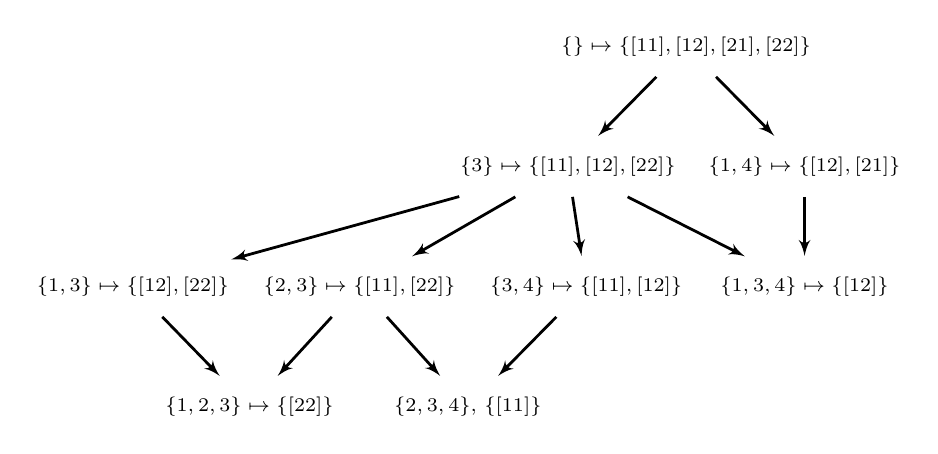
\begin{tikzpicture}[scale=.6,>=latex',line join=bevel,]

  \pgfsetlinewidth{1bp}
%%
\pgfsetcolor{black}
  % Edge: k13 -> k123
  \draw [->] (76.664bp,71.831bp) .. controls (84.973bp,63.285bp) and (95.026bp,52.944bp)  .. (111.1bp,36.413bp);
  % Edge: k23 -> k234
  \draw [->] (211.4bp,71.831bp) .. controls (219.04bp,63.369bp) and (228.27bp,53.149bp)  .. (243.38bp,36.413bp);
  % Edge: k3 -> k23
  \draw [->] (288.46bp,143.83bp) .. controls (272.32bp,134.54bp) and (252.5bp,123.12bp)  .. (226.53bp,108.16bp);
  % Edge: k -> k3
  \draw [->] (373.08bp,215.83bp) .. controls (364.66bp,207.28bp) and (354.46bp,196.94bp)  .. (338.16bp,180.41bp);
  % Edge: k34 -> k234
  \draw [->] (313.08bp,71.831bp) .. controls (304.66bp,63.285bp) and (294.46bp,52.944bp)  .. (278.16bp,36.413bp);
  % Edge: k14 -> k134
  \draw [->] (462bp,143.83bp) .. controls (462bp,136.13bp) and (462bp,126.97bp)  .. (462bp,108.41bp);
  % Edge: k3 -> k34
  \draw [->] (322.78bp,143.83bp) .. controls (323.95bp,136.13bp) and (325.35bp,126.97bp)  .. (328.19bp,108.41bp);
  % Edge: k -> k14
  \draw [->] (408.92bp,215.83bp) .. controls (417.34bp,207.28bp) and (427.54bp,196.94bp)  .. (443.84bp,180.41bp);
  % Edge: k3 -> k13
  \draw [->] (254.81bp,144.02bp) .. controls (216.12bp,133.34bp) and (167.1bp,119.82bp)  .. (118.01bp,106.28bp);
  % Edge: k23 -> k123
  \draw [->] (178.35bp,71.831bp) .. controls (170.59bp,63.369bp) and (161.22bp,53.149bp)  .. (145.88bp,36.413bp);
  % Edge: k3 -> k134
  \draw [->] (355.83bp,143.83bp) .. controls (374.42bp,134.41bp) and (397.3bp,122.81bp)  .. (426.18bp,108.16bp);
  % Node: k13
\begin{scope}
  \definecolor{strokecol}{rgb}{0.0,0.0,0.0};
  \pgfsetstrokecolor{strokecol}
  \draw (59bp,90bp) node {\scriptsize$\{1,3\}\mapsto\{[12],[22]\}$};
\end{scope}
  % Node: k34
\begin{scope}
  \definecolor{strokecol}{rgb}{0.0,0.0,0.0};
  \pgfsetstrokecolor{strokecol}
  \draw (331bp,90bp) node {\scriptsize$\{3,4\}\mapsto\{[11],[12]\}$};
\end{scope}
  % Node: k14
\begin{scope}
  \definecolor{strokecol}{rgb}{0.0,0.0,0.0};
  \pgfsetstrokecolor{strokecol}
  \draw (462bp,162bp) node {\scriptsize$\{1,4\}\mapsto\{[12],[21]\}$};
\end{scope}
  % Node: k23
\begin{scope}
  \definecolor{strokecol}{rgb}{0.0,0.0,0.0};
  \pgfsetstrokecolor{strokecol}
  \draw (195bp,90bp) node {\scriptsize$\{2,3\}\mapsto\{[11],[22]\}$};
\end{scope}
  % Node: k
\begin{scope}
  \definecolor{strokecol}{rgb}{0.0,0.0,0.0};
  \pgfsetstrokecolor{strokecol}
  \draw (391bp,234bp) node {\scriptsize$\{\}\mapsto\{[11],[12],[21],[22]\}$};
\end{scope}
  % Node: k234
\begin{scope}
  \definecolor{strokecol}{rgb}{0.0,0.0,0.0};
  \pgfsetstrokecolor{strokecol}
  \draw (260bp,18bp) node {\scriptsize$\{2,3,4\}$, \{[11]\}};
\end{scope}
  % Node: k3
\begin{scope}
  \definecolor{strokecol}{rgb}{0.0,0.0,0.0};
  \pgfsetstrokecolor{strokecol}
  \draw (320bp,162bp) node {\scriptsize$\{3\}\mapsto\{[11],[12],[22]\}$};
\end{scope}
  % Node: k123
\begin{scope}
  \definecolor{strokecol}{rgb}{0.0,0.0,0.0};
  \pgfsetstrokecolor{strokecol}
  \draw (129bp,18bp) node {\scriptsize$\{1,2,3\}\mapsto\{[22]\}$};
\end{scope}
  % Node: k134
\begin{scope}
  \definecolor{strokecol}{rgb}{0.0,0.0,0.0};
  \pgfsetstrokecolor{strokecol}
  \draw (462bp,90bp) node {\scriptsize$\{1,3,4\}\mapsto\{[12]\}$};
\end{scope}
%
\end{tikzpicture}

\end{figure}

\section{Conclusion}

\begin{tabular}{|l|c|c|c|c|c|}
\hline
$n$ & 0 & 1 & 2 & 3 & 4 \\
\hline
$S_n$ & - & 1,1 & 2,2 & 6,4 & 30,11\\
\hline
$T_n$ &1,1 & 2,2 & 10,8 & 1299,283 & \\
\hline
$T_n\setminus S_n$ & 1,1 & 1,1 & 4,3 & 600,123& \\
\hline
\end{tabular}
\todo{check reference Dietlinde Lau, T3 partially, 1982}
\bibliographystyle{plain}
\bibliography{subsemicut}
\end{document}
